%!TEX root = ../dissertation.tex

\chapter{Experiment 2: Effect of Retinal Eccentricity on Fixational Stability and Accuracy}

\section{Brief Introduction}

Experiment 2 follows Experiment 1 quite naturally in that it examines the effect of the other major parameter that characterizes pPRLs: eccentricity relative to the fovea. Unlike with orientation, there is a strong consensus in the literature that functional vision performance decreases sharply and continuously as a function of increased eccentricity\citep{carrasco_2001,whittaker_1988}. What is more, patients with newly formed macular scotoma seem to unconsciously select PRL close to the border of the scotoma\citep{cummings_1985,timberlake_1986} (and thus to the site of the former fovea), implying that the brain is capable of responding to and selecting against some form of feedback that marks reduced performance in the visual periphery. The two primary research questions this experiment is designed to address are:

\begin{enumerate}
\item Will increased eccentricity relative to the fovea reduce fixational stability and accuracy improvements associated with the development of a pPRL?
\item Do changes in retinal eccentricity impair pPRL learning/retention?
\end{enumerate}

\section{Methods}

The methods, experimental setup, and design for this experiment are effectively identical to those used in Experiment 1. Subjects' task, the stimulus, the test-retest design of the first experiment, and the variables of interest were all carried over to this experiment. However, because of apparent asymptotes in gains associated with the use of the training program, the number of trials in each training set was reduced from 200 to 100. Trials were otherwise still completed in sets of fifty with mandatory breaks and recalibration of the eye tracking system between blocks. The experimental manipulations in this case were two eccentricity conditions: a ‘near’ condition that placed the gaze-contingent ring 6.4\degree (128 pix) to the right of the foveated point of regard, and a ‘far’ condition which increased this distance by a factor of 1.75 to 11.2\degree (224 pix) (see Figure ~\ref{chap_2_demo_figure}). The order in which subjects completed the eccentricity conditions was counter-balanced between subjects. Five women and three men, all undergraduates at Northeastern University, completed both conditions. There was an average of ~8 days sd(~1) between subjects' first and second training sessions.

\begin{figure}[!htbp]
\centering
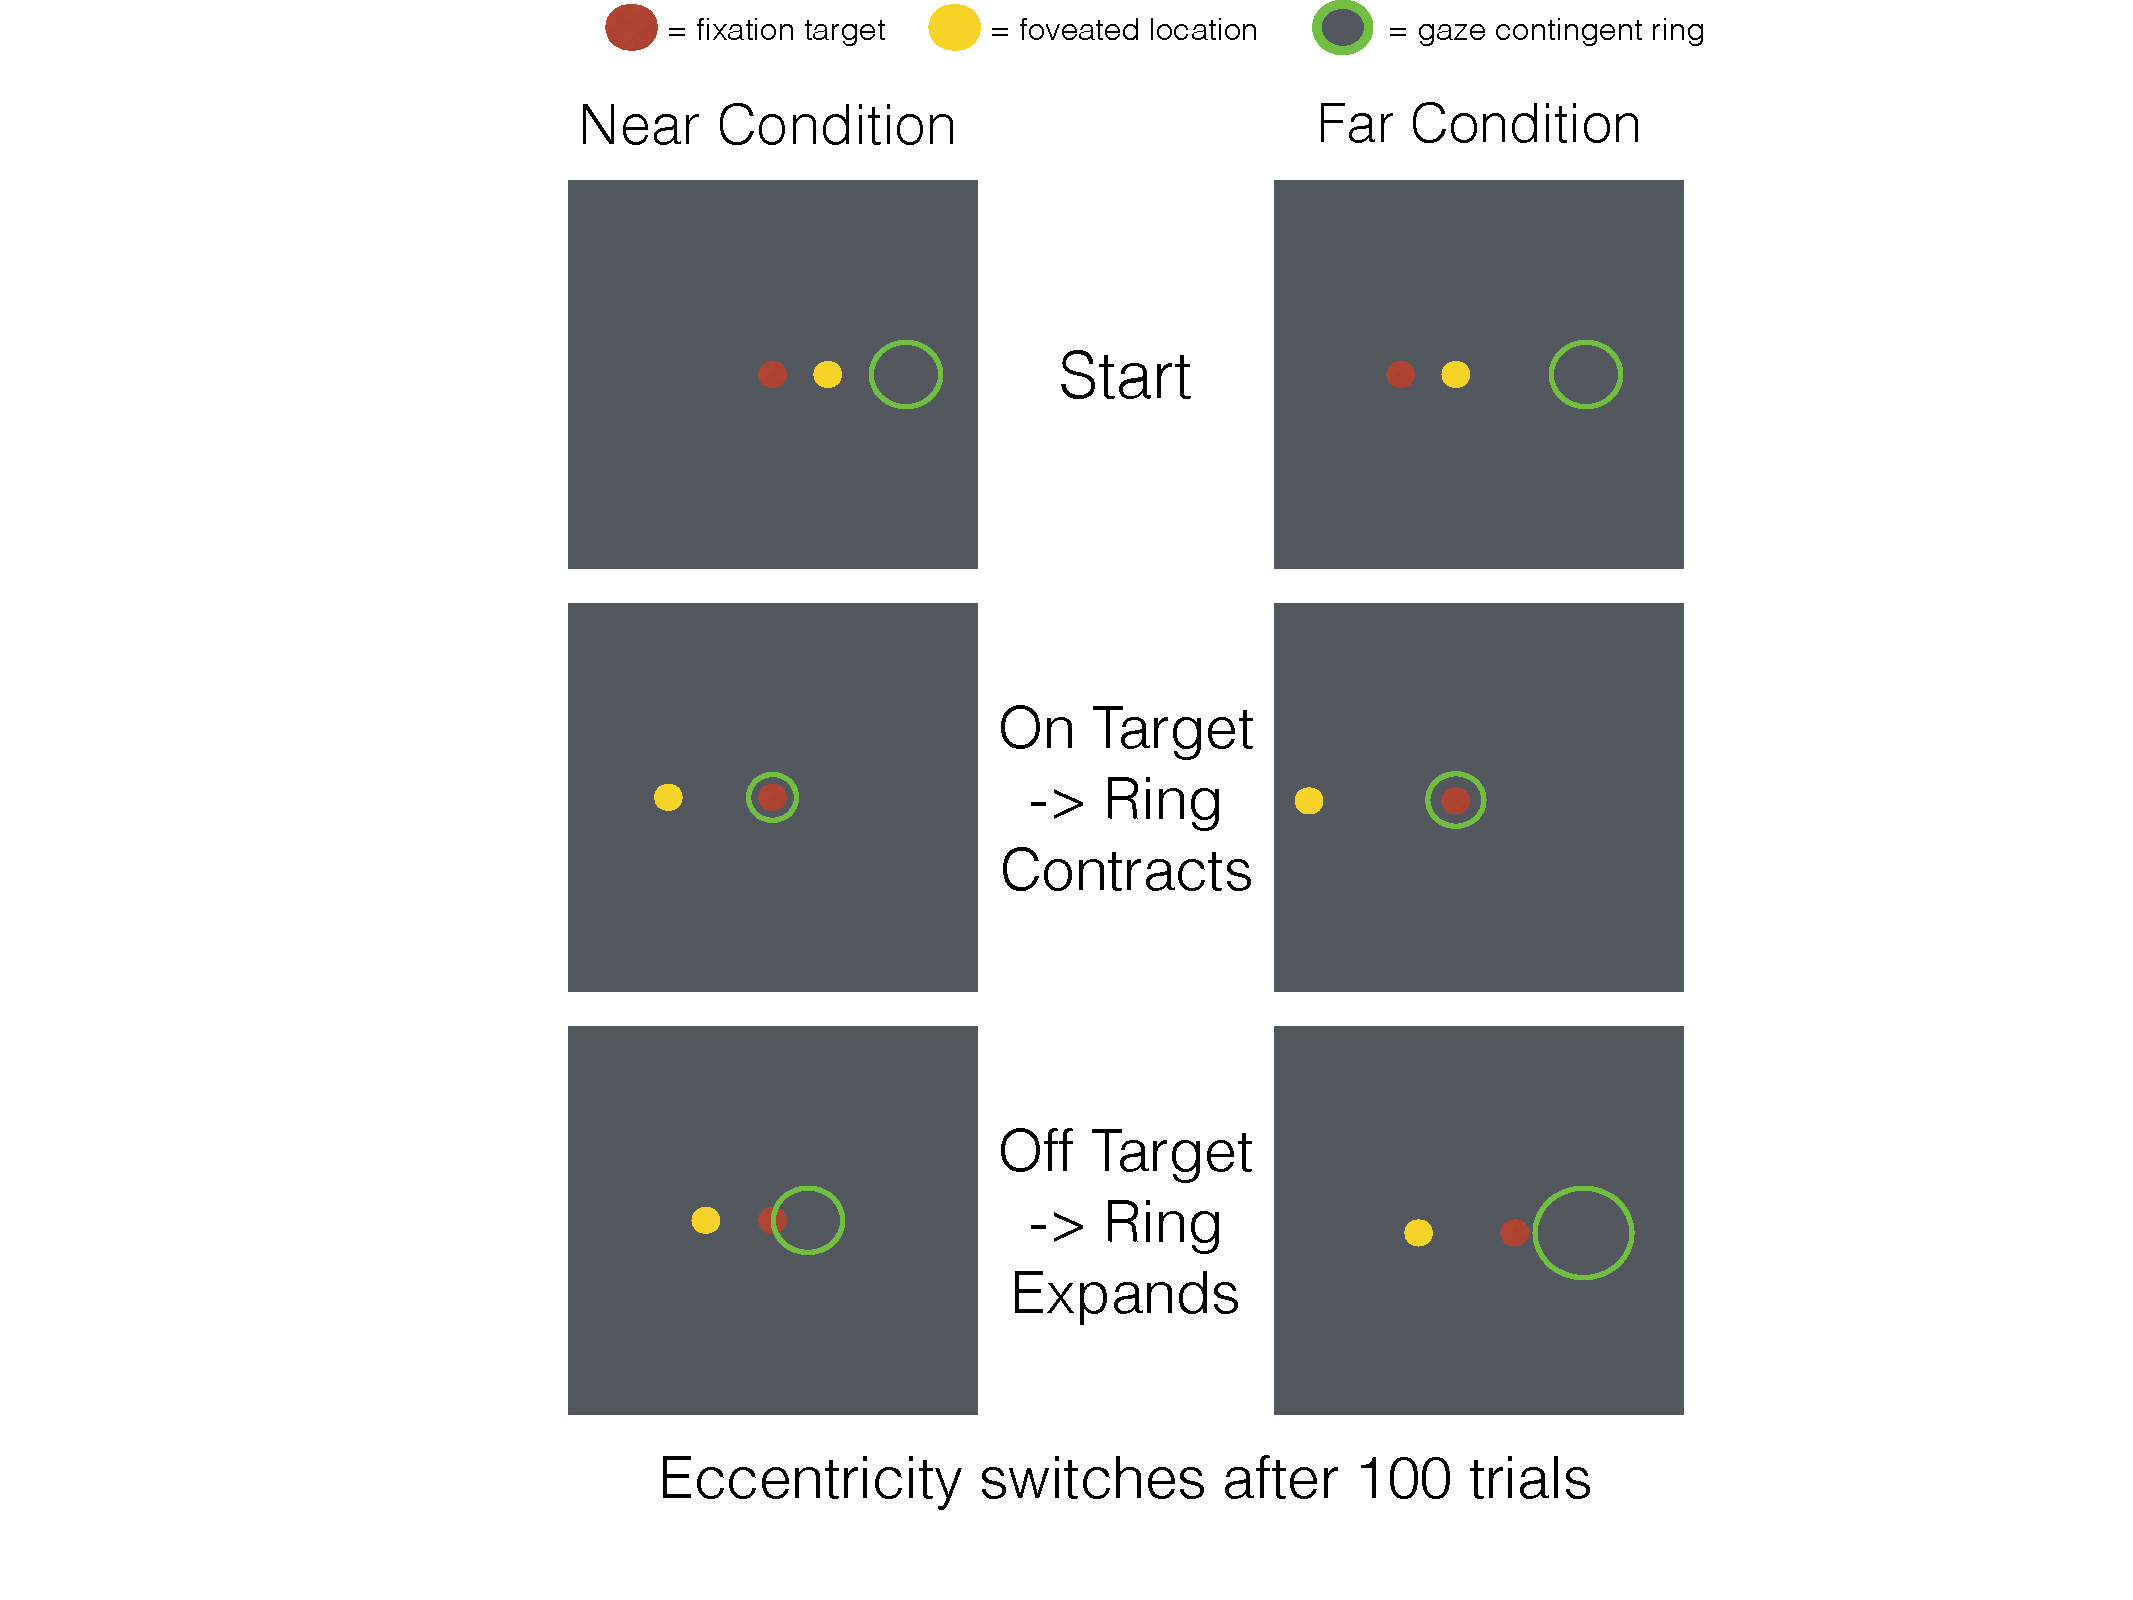
\includegraphics[width=.75\linewidth,height=.75\textheight,keepaspectratio]{figures/chapter_2/eccentricity_demo.pdf}
\caption[Schematic Depiction of Experimental Design for Experiment 2]{Subjects completed a training session composed of 100 trials in one eccentricity condition, then completed a second session in the other approximately a week later. Keeping the ring on target caused it to contract after 100ms, making the task harder. Falling off target during the same period caused it to expand, making the task easier. Recorded foveal position (yellow circle) was not shown to research participants.}\label{chap_2_demo_figure}
\end{figure}

\section{Results}

Figure ~\ref{chap_2_outcome_by_block} shows performance patterns across subjects for all four blocks of training. As with the data for Experiment 1, a broad pattern of improvement across blocks is visible. Unlike in Experiment 1, however, both accuracy and stability performance appear to have been much better retained following the inter-session gap. This interpretation is largely supported by the fitted HLM model parameters (Table ~\ref{chap_2_model_fit}. As in Experiment 1, a significant main effect of block number (coefficient: -0.330, \textit{p}\textless0.01) on accuracy was observed. Subjects' accuracy with respect to the target therefore generally improved across training blocks. In this case, however, a main effect of training set (i.e., whether the data were taken from the first or second set of blocks) was also observed. Specifically, data from the second training set was on average nearly a full log-unit higher than the first. Stability performance did not show a similar reduction in performance when subjects returned for the second training session. In this case, only the parameter for absolute block number reached statistical significance (coefficient: -110,649.30,\textit{p}\textless0.05).

\begin{figure}[htbp]
\centering
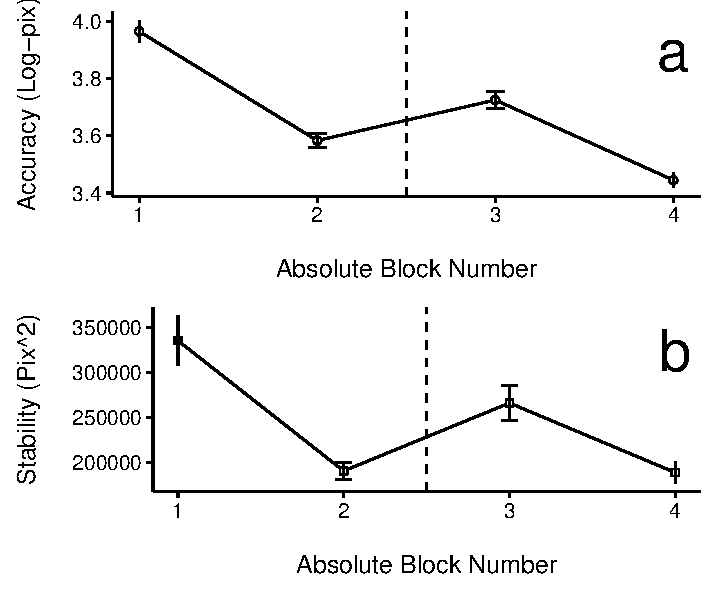
\includegraphics[width=.75\linewidth,height=.75\textheight,keepaspectratio]{figures/chapter_2/outcome_by_block.pdf}
\caption[Experiment 2: Outcomes by Block]{\textbf{a}: log-transformed median distance (pixels) between the centers of the target and ring as a function of training block number across subjects and trials. Dots represent within block means, and bars 95\% confidence intervals. The dashed line between blocks 2 and 3 on the x-axis is the point at which subjects switched orientation conditions. \textbf{b}: mean stability performance (pixels-squared) within blocks and across subjects. The elements of this figure are otherwise the same as in \textbf{a}.}\label{chap_2_outcome_by_block}
\end{figure}

\begin{table}[!htbp] \centering
\resizebox{.75\linewidth}{!}{\begin{minipage}{\linewidth}
  \caption{Experiment 2: Outcome Model Fits} 
  \label{chap_2_model_fit} 
\begin{tabular}{@{\extracolsep{5pt}}lcc} 
\\[-1.8ex]\hline 
\hline \\[-1.8ex] 
 & \multicolumn{2}{c}{\textit{Dependent variable:}} \\ 
\cline{2-3} 
\\[-1.8ex] & Accuracy (Log Pixels) & Stability (Pixels Squared) \\ 
\\[-1.8ex] & (1) & (2)\\ 
\hline \\[-1.8ex] 
 Absolute Block Number & $-$0.330$^{***}$ & $-$110,649.300$^{**}$ \\ 
  & (0.089) & (44,153.960) \\ 
  Eccentricity Condition & 0.377 & 35,284.820 \\ 
  & (0.411) & (124,363.900) \\ 
  First or Second Training Session & 0.852$^{**}$ & 189,483.200 \\ 
  & (0.411) & (121,142.100) \\ 
  Eccentricity x First or Second Training Session& $-$0.761 & $-$7,195.719 \\ 
  & (0.815) & (232,943.600) \\ 
 \hline \\[-1.8ex] 
Observations & 1,600 & 1,600 \\ 
Log Likelihood & $-$1,079.776 & $-$22,407.140 \\ 
Akaike Inf. Crit. & 2,177.552 & 44,832.280 \\ 
Bayesian Inf. Crit. & 2,225.952 & 44,880.680 \\ 
\hline 
\hline \\[-1.8ex] 
\textit{Note:}  & \multicolumn{2}{r}{$^{*}$p$<$0.1; $^{**}$p$<$0.05; $^{***}$p$<$0.01} \\ 
\end{tabular}
\end{minipage} } 
\end{table} 

Finally, a set of paired t-tests comparing outcomes in block 1 to block 3 were performed to assess the degree of training retention between sessions. Both accuracy (\textit{t}\textdblhyphenchar5.15,\textit{p}\textless0.001,\textit{df}\textdblhyphenchar399) and stability (\textit{t}\textdblhyphenchar2.23,\textit{p}0.001,\textit{df}\textdblhyphenchar399) were significantly better during block 3 than block 1, again supporting the claim that performance was effectively retained between training sessions than in Experiment 1 (see Figure~\ref{chap_2_paired_t}).

\begin{figure}[htbp]
\centering
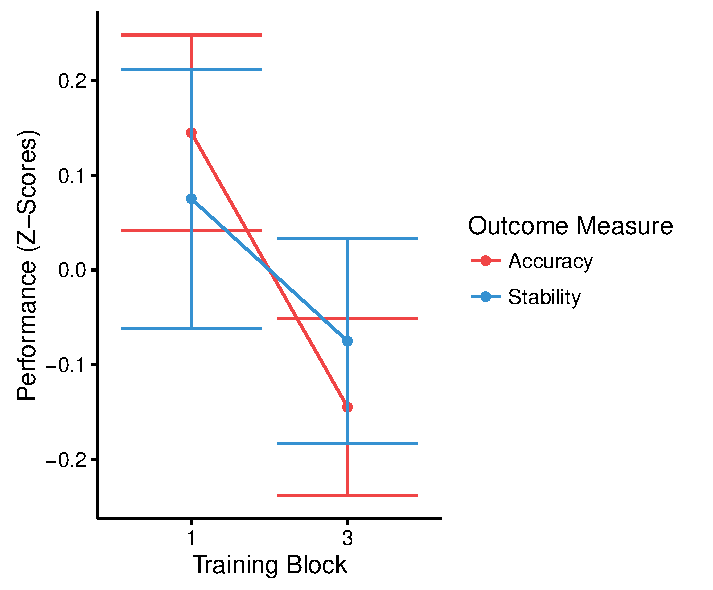
\includegraphics[width=.75\linewidth,height=.75\textheight,keepaspectratio]{figures/chapter_2/paired_t_results.pdf}
\caption[Experiment 2: Performance Comparison Between First Block of Both Sessions for Both Outcome Measures]{Means and 95\% confidence intervals for outcome measures 95\% fitted isocontour areas) between training block 1 (the first block of the first session) and training block 5 (the first block of the second training session). Data in this figure have been transformed to z-scores (mean zero, standard deviation of one) in order to set them on a shared scale.}\label{chap_2_paired_t}
\end{figure}

\section{Brief Discussion}

Results from Experiment 2 were generally well aligned with those of Experiment 1. Again, fixational stability and accuracy both improved significantly across training sessions and despite either a doubling or a halving of the distance between the fovea and the pPRL site between sessions. However, the most interesting result was the absence of a main effect of training session for the stability data. This implies that, unlike with orientation shifts, eccentricity shifts seem to make less of an impact in terms of the retention of performance without supplementary practice. As stability is to some extent the outcome measure that is more likely to have a meaningful impact on functional visual performance, and because it is also the one less specifically tied to the structure of the training exercise, this is encouraging for the ultimate impact of our method.
